% =====================================================================
% Chapter 2: Background
%
% Required topic: a critical review of the methods and the knowledge
% that exist at the time of writing, together with Chapter 3. This
% chapter carries the knowledge the thesis builds on, and Chapter 3
% reviews the methods that address the same problem.
%
% Every definition the thesis uses belongs here, so that Chapter 4
% only has to state the purposes of the research. The first three
% sections are the Background section of the paper; the fourth has no
% counterpart there, as the paper assumes the abstractions known.
%
% fig_delta.pdf is copied from the figures of the paper.
% =====================================================================
\chapter{Preliminaries}
\label{ch:background}

In this chapter, we present the background this thesis builds on. We
begin with neural network classifiers, continue with global
robustness, and close with its exact verification.

\section{Neural Network Classifiers}
\label{sec:background-networks}

We consider neural network classifiers
$N : \reals^{n} \to \reals^{|C|}$, where $n$ is the input dimension and
$C$ the set of classes. Inputs are assumed to lie in $[0,1]^n$, as is
standard for image classifiers. An input $x$ is classified by its
maximal score, $c = \mathrm{argmax}(N(x))$. The network has an input
layer $z_{0,k} = x_k$ followed by $L$ layers, such that $N(x) = \hat{z}_L$. 
Every neuron computes a \emph{pre-activation}, 
an affine expression over the neurons of the
previous layer, and every layer but the last one follows it with an
\emph{activation}, a non-linear function applied to it. We consider two kinds
of layers: fully connected and convolutional.

\paragraph{Fully connected layers.}
We write $z_{m,k}$ for the $k$th neuron of layer $m$ and $k_m$ 
for its number of neurons. Its
pre-activation weights every neuron of the previous layer by
$w_{m,k,k'}$ and adds a bias $b_{m,k}$:
\begin{equation}
  \hat{z}_{m,k} = b_{m,k}
  + \sum_{k'=1}^{k_{m-1}} w_{m,k,k'} \cdot z_{m-1,k'}.
  \label{eq:pre-activation}
\end{equation}

\paragraph{Convolutional layers.}
We write $z_{m,i,j,d}$ for the neuron at the row $i$, the column $j$
and the channel $d$ of layer $m$, and $d_m$ for the number of channels
the layer has. Its pre-activation weights a local region
of the previous layer by a kernel $W_m$ of size $t_m \times t_m$ per
channel, slid in steps of a stride $s_m$, and adds the bias $b_{m,d}$
of the channel:
\begin{equation}
  \hat{z}_{m,i,j,d} = b_{m,d} + \sum_{p=1}^{t_m} \sum_{q=1}^{t_m}
  \sum_{v=1}^{d_{m-1}} W_m[p,q,v,d] \cdot
  z_{m-1,\,(i-1)s_m+p,\,(j-1)s_m+q,\,v}.
  \label{eq:pre-activation-conv}
\end{equation}

\paragraph{Activation.}
Every layer but the last one is followed by an activation, the same
for both kinds of layers, and we focus on ReLU, one of the most
popular activation functions:
\begin{equation}
  z_{m,k} = \relu(\hat{z}_{m,k}) = \max(0, \hat{z}_{m,k}).
  \label{eq:relu}
\end{equation}
Where the layout of a layer does not matter, we number its neurons
with the single index $k$ of~\eqref{eq:pre-activation}, whether the
layer is fully connected or convolutional, as
in~\eqref{eq:relu}.

\section{Global Robustness}
\label{sec:background-robustness}

\begin{figure}[t]
\centering
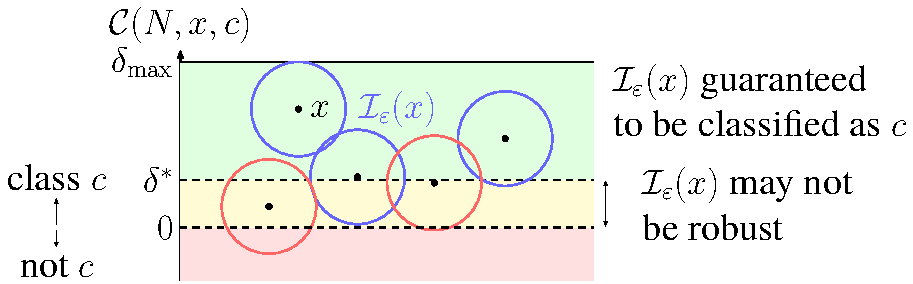
\includegraphics[width=0.75\linewidth]{fig_delta}
\caption{Illustration of the minimal globally robust bound.}
\label{fig:delta}
\end{figure}

Intuitively, given a perturbation type with a bounded size, a network
$N$ is \emph{$\delta$-globally robust} for a class $c$ if every input
it classifies as $c$ with confidence at least $\delta$ stays
classified as $c$ under that perturbation~\citep{kabaha2024vhagar}.
Since the confidence of a network is bounded by some $\delta_{\max}$,
every network is $\delta_{\max}$-globally robust; the goal is to
compute the minimal globally robust bound, denoted $\delta^*$, as it
flags the fewest inputs as potentially unsafe.
Figure~\ref{fig:delta} illustrates this, plotting each input $x$ as a
black dot at its confidence for the class $c$, along with its
neighborhood of perturbed inputs as a circle. An input with confidence
below $0$ is not classified as $c$, on the red background; one with
confidence below the globally robust bound $\delta^*$ may have a
perturbed input with confidence below $0$, and is thus not guaranteed
robust, on the yellow background; and one with confidence at least
$\delta^*$ stays classified as $c$ under every perturbation, on the
green background.

Formally, the \emph{confidence} of an input $x$ in a class $c$ is the
gap between its score and the next-highest one:
\begin{equation}
  \conf{N}{x}{c} := N(x)_c - \max_{k \neq c} N(x)_k,
  \label{eq:confidence}
\end{equation}
and $N$ classifies $x$ as $c$ when $\conf{N}{x}{c} > 0$. A
\emph{perturbation} is a function $P$ that, given an input $x$ and a
size $e$, returns a perturbed input, and we denote the set of all
perturbations of $x$ up to size $\ep$ by
\begin{equation}
  \mI_\ep(x) = \{P(x, e) \mid e \leq \ep\}.
  \label{eq:perturbation-set}
\end{equation}
The minimal globally robust bound $\delta^*$ is defined by adding a
small number to its counterpart, the \emph{maximal non-robust bound}.
We define this bound as the maximum of $\hat{\delta}_{c_t}$ over all
target classes $c_t \neq c$, where
\begin{equation}
\begin{aligned}
  \hat{\delta}_{c_t} = \max\; \bigl\{\, \delta \;\bigm|\;
  &\exists x,\, x^{p} \in \mI_\ep(x): \\
  &\conf{N}{x}{c} \geq \delta \,\wedge\, \conf{N}{x^{p}}{c_t} > 0
  \,\bigr\}.
\end{aligned}
\label{eq:max-non-robust-bound}
\end{equation}
Namely, it is the highest confidence at which some input classified as
$c$ can still be perturbed into $c_t$.

\section{Exact Verification}
\label{sec:background-exact-verification}

\tool accelerates exact analysis that relies on constraint solving.
Such analysis defines the confidences $\conf{N}{x}{c}$ and
$\conf{N}{x^{p}}{c_t}$ over an input $x$ and its perturbation
$x^{p} \in \mI_\ep(x)$ through constraints, for example in first-order
logic~\citep{katz2019,katz2017reluplex} or in a mixed-integer
program~\citep{tjeng2019}. A solver then computes
\[
  \hat{\delta}_{c_t} = \max \conf{N}{x}{c}
  \quad \text{subject to} \quad
  \conf{N}{x^{p}}{c_t} > 0 .
\]

To encode $\conf{N}{x}{c}$, the analysis introduces for each neuron a
variable for its pre-activation $\hat{z}_{m,k}$ and one for its ReLU
output $z_{m,k}$, and adds constraints capturing their functions.
Similarly, to encode $\conf{N}{x^{p}}{c_t}$, it introduces
$\hat{z}^{p}_{m,k}$ and $z^{p}_{m,k}$, so it has two copies of the
network. As is common, it also computes an interval bounding each
affine part, $[l_{m,k}, u_{m,k}]$ for the copy on $x$ and
$[l^{p}_{m,k}, u^{p}_{m,k}]$ for the copy on $x^{p}$, by optimization or
by interval propagation. These intervals identify the ReLUs whose
function is linear, when $u_{m,k} \leq 0$ or $l_{m,k} \geq 0$, in
which case $z_{m,k}$ is $0$ or $\hat{z}_{m,k}$ and a single linear
constraint encodes it. We call such a neuron \emph{stable}. The
remaining ReLUs, those with $l_{m,k} < 0 < u_{m,k}$, are
\emph{unstable}: each of them is encoded with a
binary variable $a_{m,k}$, which is $1$ when the neuron is active and
$0$ when it is inactive, together with the four constraints of
\citet{tjeng2019}:
\begin{equation}
\begin{aligned}
  z_{m,k} &\geq 0, &\qquad
  z_{m,k} &\geq \hat{z}_{m,k}, \\
  z_{m,k} &\leq u_{m,k}\, a_{m,k}, &\qquad
  z_{m,k} &\leq \hat{z}_{m,k} - l_{m,k}(1 - a_{m,k}).
\end{aligned}
\label{eq:relu-encoding}
\end{equation}
When $a_{m,k}$ is $1$ the neuron is active and
$z_{m,k} = \hat{z}_{m,k}$, and when it is $0$ the neuron is inactive
and $z_{m,k} = 0$. The complexity of the problem is therefore
exponential in the number of unstable neurons.

Solving this program exactly is expensive, so a verifier is run with a
timeout. An anytime solver maintains bounds $\dlo$ and $\dup$ on the
optimum $\hat{\delta}_{c_t}$, tightening both as it searches, and
stopping it at any point gives the sound guarantee
$\hat{\delta}_{c_t} \in [\dlo, \dup]$. The two bounds meet at
optimality, and the narrower the interval, the more the analysis has
established, which is why we report it alongside the execution time.
